\documentclass{article}

% ready for submission
\usepackage[final]{neurips_2021}
\usepackage[utf8]{inputenc} % allow utf-8 input
\usepackage[T1]{fontenc}    % use 8-bit T1 fonts
\usepackage{hyperref}       % hyperlinks
\usepackage{url}            % simple URL typesetting
\usepackage{booktabs}       % professional-quality tables
\usepackage{amsfonts}       % blackboard math symbols
\usepackage{nicefrac}       % compact symbols for 1/2, etc.
\usepackage{microtype}      % microtypography
\usepackage{xcolor}         % colors
\usepackage{enumitem}
\usepackage{algorithm}
\usepackage{algpseudocode}
\usepackage{fancyhdr}
\usepackage{graphicx}
% \usepackage{comment}

%\usepackage[T1]{fontenc}    % use 8-bit T1 fonts
%\usepackage{hyperref}       % hyperlinks
%\usepackage{url}            % simple URL typesetting
%\usepackage{booktabs}       % professional-quality tables
%\usepackage{amsfonts}       % blackboard math symbols
%\usepackage{nicefrac}       % compact symbols for 1/2, etc.
%\usepackage{microtype}      % microtypography
%\usepackage[dvipsnames]{xcolor}        % colors

%\usepackage[utf8]{inputenc}
%\usepackage{multicol,multirow}
%\usepackage{amsmath}
%\usepackage[legalpaper, margin=1in]{geometry}


\title{CS271 Project Draft Design: Sokoban}

\author{
  Nitya Raju\\
  Department of Computer Science\\
  University of California, Irvine\\
  Irvine, CA 92697\\
  \texttt{nraju1@uci.edu} \\
   \And
  Akshita Singh \\
  Department of Computer Science\\
  University of California, Irvine\\
  Irvine, CA 92697\\
  \texttt{akshis2@uci.edu} \\
   \And
  Almendra Salgado Gatica \\
  Department of Computer Science\\
  University of California, Irvine\\
  Irvine, CA 92697\\
  \texttt{arsalgad@uci.edu} \\
}
\begin{document}

\maketitle

%\begin{abstract}
    
%  The abstract paragraph should be indented \nicefrac{1}{2}~inch (3~picas) on
%  both the left- and right-hand margins. Use 10~point type, with a vertical
%  spacing (leading) of 11~points.  The word \textbf{Abstract} must be centered,
%  bold, and in point size 12. Two line spaces precede the abstract. The abstract
%  must be limited to one paragraph.
%\end{abstract}

\section{Introduction}

Sokoban is a part puzzle, part video game in which a player (Sokoban) pushes around boxes such that they end up in storage locations which are pre-determined by a game level. Sokoban runs into walls and other boxes along the way and whether or not it can navigate its way around such roadblocks is what forms the crux of this game. We have developed an AI agent for Sokoban. Our project aims to develop a reasonably intelligent AI Sokoban that can handle multiple configurations of walls, boxes, and storages, all with varying complexities. To make this happen, we called on to the Q-Learning algorithm from within the larger umbrella of Reinforcement Learning and Markov Decision Processes. Besides that, we invested in identifying some efficient approaches to identifying as many deadlock scenarios as possible, if not all. 

% \section{Reinforcement Learning and Q- Learning}
% \textbf{What is Reinforcement Learning?}: \\
% Reinforcement Learning (RL) essentially entails decision making in an unknown and stochastic environment. To support this decision making, we call on to some of the following elements of RL: \emph{Rewards, Value Functions, Policies}. For Sokoban, this Rewards would look something like this: 

% a) (+100) for a move that leads to a ("win"

% b) (-100) for a move that creates a deadlock

% c) (-10) for a move that kicks a box out of a storage location

% d) (+10) for a move that pushes a box into a storage location

% e) (+5) for a move that pushes a box without creating a deadlock**

% f) (-1) for a move into empty square that does not create a deadlock***
% \\
% * Win: the move that pushes the last remaining box not in a storage location into a storage location \\
% ** Deadlock: a deadlock that we have been able to capture \\
% *** We do penalize a move with a negative score even if its in the right direction, because our goal is to push the boxes into storage locations as quickly as possible. \\
% \\
% RL algorithms can be broken down based on whether they are model-dependent or model-free. For Markov Decision Processes (MDP) the "model" largely consists of state transition probabilities and rewards: $<S, A, P, R, \gamma>$. Temporal Difference Leaning (TD) is the subset of RL algorithms that do not have these transition probabilities and rewards explicitly defined. Learning happens through "episodes of experience". The two common algorithms within TD are Q-Learning and SARSA. 
% \\
% \\
% \textbf{What is Q-Learning?}:
% Q-Learning is a TD algorithm that learns action values relative to the greedy policy. A Q-Learning algorithm follows the greedy policy with with some probability < epsilon, and the optimal policy with the probability (1 - epsilon). This is in contrast to SARSA, which learns action values relative to the policy it follows. \\
% % SARSA: $Q(S,A) \leftarrow Q(S,A) + \alpha(R + \gamma Q(S',A') - Q(S,A))$ \\
% Q-Learning: $Q(S,A) \leftarrow Q(S,A) + \alpha(R + \gamma max_{\alpha'}Q(S',A') - Q(S,A))$  \\
% where: \\
% $S$ is the current state  \\
% $A$ is the current action \\
% $S'$ is the next state \\
% $A'$ is the next action \\
% $R$ is the reward \\
% $\alpha$ is the discount rate \\
% $\gamma$ is the learning rate \\
% $Q(S,A)$ is the Action Function at the current state $S$ with current action $A$ \\
% $Q(S',A')$ is the Action Function at the next state $S'$ with next action $A'$ \\
% \\
% \\
% \textbf{Why Q-Learning}
% Sokoban is a puzzle with very few consistencies to exploit. Our AI Sokoban has no idea where the walls, boxes, and storage locations would be as we take it from one level to another. The real "reward" is successfully pushing all boxes in storage locations. Thus Sokoban is a game with sparse rewards and not much information and consistencies to with. This makes it apt for an algorithm that learns and improves along the way, instead of waiting for the whole episode to get over to learn anything at all. \\ \\
% At each step, Q Learning computes the error after learning from a policy outside its domain $\alpha(R + \gamma max_{\alpha'}Q(S',A') - Q(S,A))$ and updates $Q(S,A)$ accordingly. Because Q-Learning does not follow an policy, it can continue learning while changing policies. This flexibility of changing policies and hence ensuring optimality is what drew us towards Q-Learning as against SARSA. 

\section{Approach To Game Development}

We modularised our program and broke it down into 3 classes: 1) Agent, 2) State, and 3) Game.

\subsection{Agent}
The Agent class focused on the actions Sokoban would take given the rules of the game and the constraints of Q Learning Algorithm. We included 3 principal methods in this class:
    
\begin{enumerate}[label=\alph*)]
    \item \underline{AgentMove}: This function returns the action Sokoban takes using an $\epsilon$-greedy policy. This means Sokoban takes a random action with probability $\epsilon$ (initialized to $0.1$) and acts according to the policy it learns the remaining time. The pseudo-code for the same is described in detail in the next section.
    \item \underline{MovePlayer}: This function implement Sokoban's move given the rules of the game. It looks into the surrounding region once the agent takes an action and informs the game of any boxes Sokoban moved, or any obstacles (walls, deadlocks, bounds) that it confronted along the way. 
    \item \underline{qValueUpate}: This function updates the current q-value by loyally following the Q-Learning algorithm formula. The pseudo-code for this function is also detailed out in the next section. 
\end{enumerate}

\subsection{State}
The state class plays the important role of deciding the fate of Sokoban given the level it has been placed into. It takes the level parameters (coordinates of the agent, walls, boxes, and goals) to construct the initial board. And with that information, Sokoban decides how to go about getting to the goal as quickly possible, with the help of the Agent class. We included 3 principal methods in this class: 

\begin{enumerate}[label=\alph*)]
    \item \underline{createBoard}: This function creates the structure of the board as specified by the project specifications. 
    \begin{enumerate}
        \item '\#' corresponds to a wall
        \item '\$' corresponds to a box
        \item '.' corresponds to a storage location
        \item '@' corresponds to the agent location
    \end{enumerate}
    For example, for the below project specification, we will generate the below board.  
    \begin{figure}[htp]
        \centering
        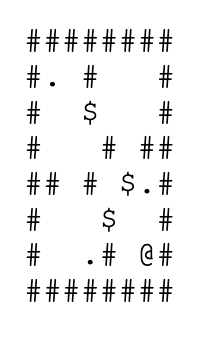
\includegraphics[width=5cm]{Input.png}
        \caption{Input Board}
    \end{figure} 
    \begin{figure}[htp]
        \centering
        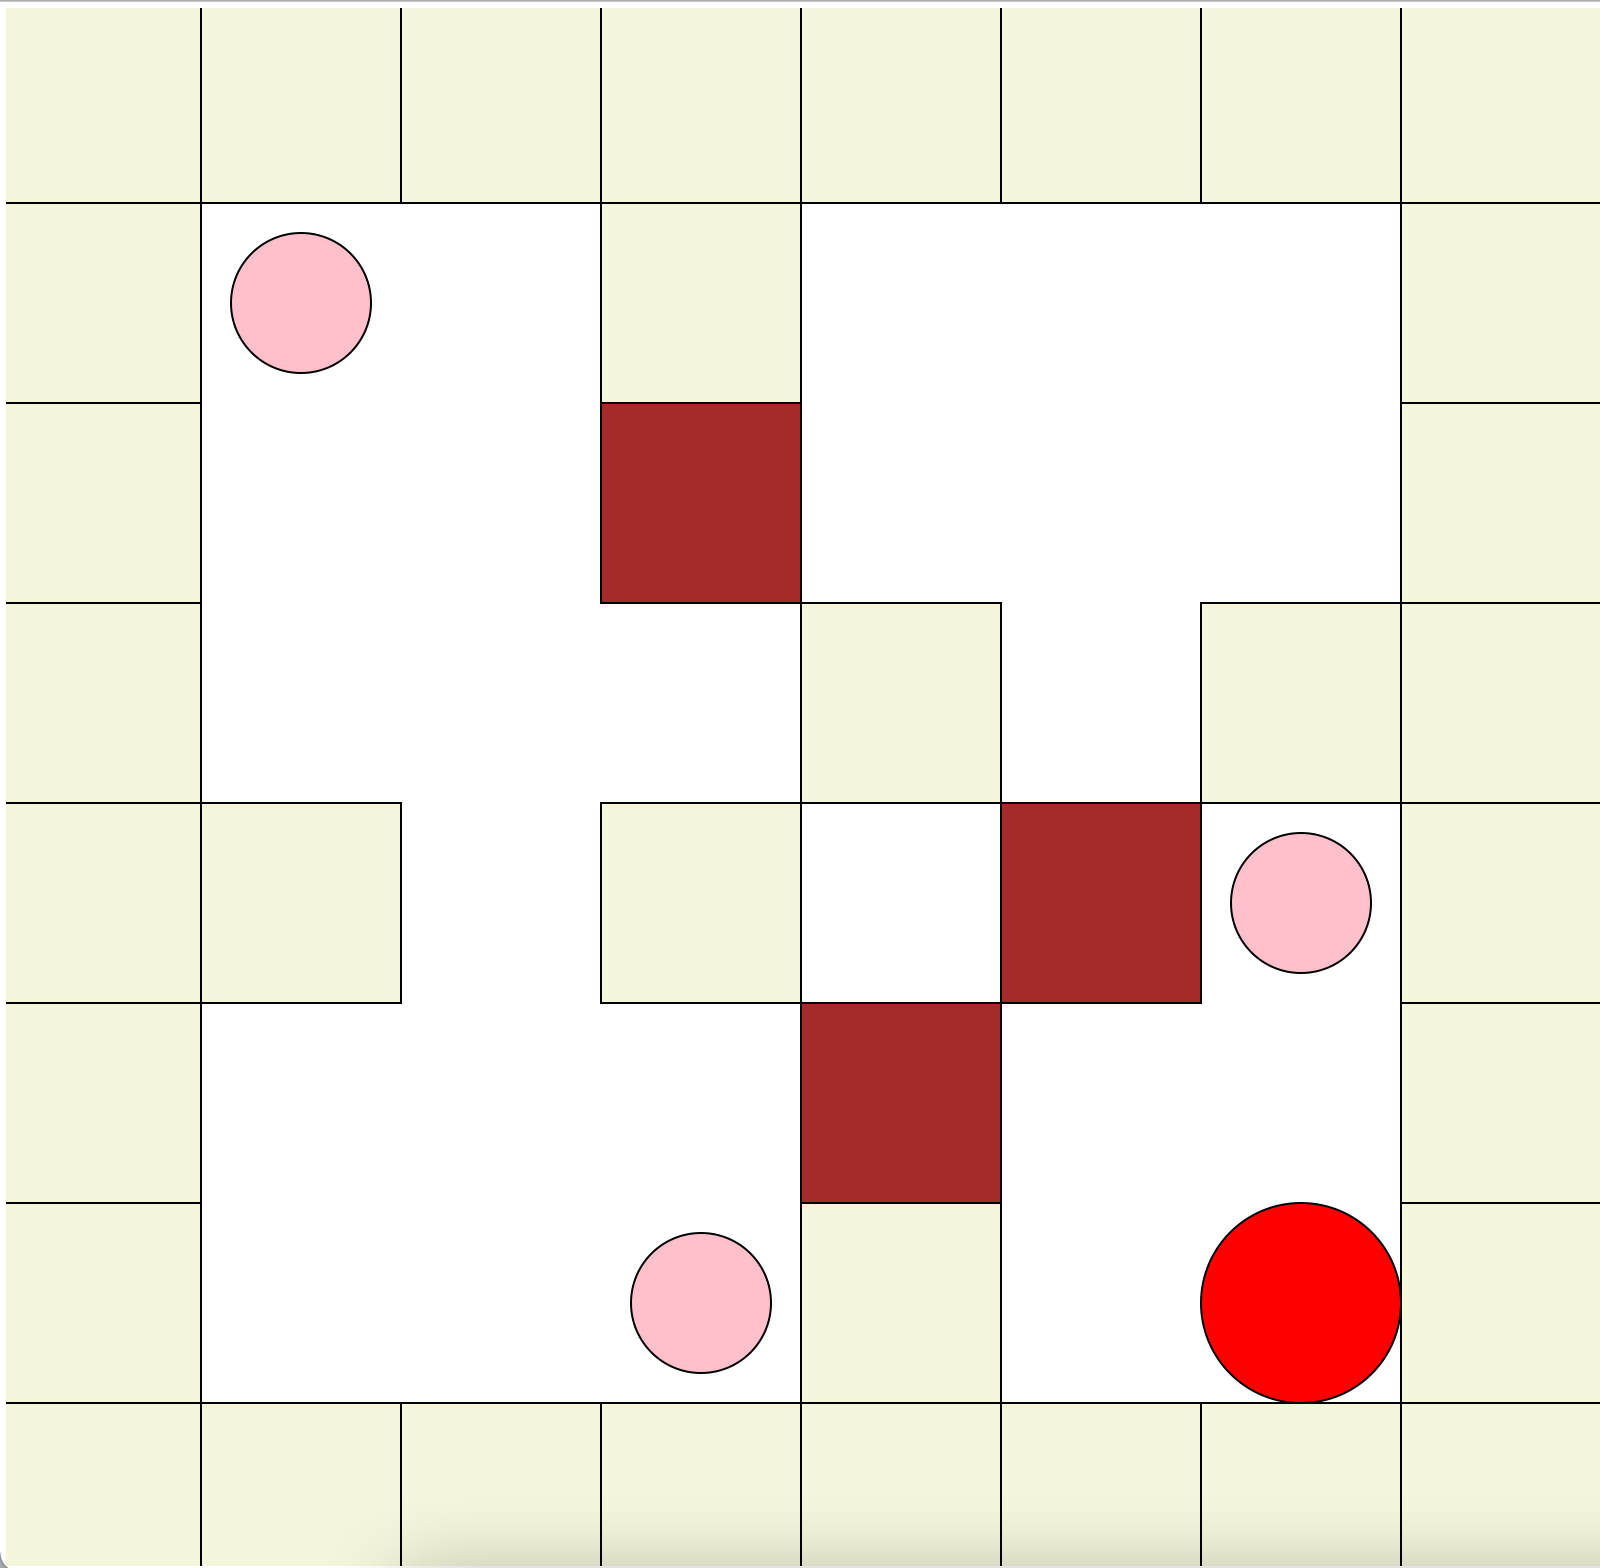
\includegraphics[width=5cm]{Board.png}
        \caption{Initial State of Board}
\end{figure} 
    \item \underline{checkBoard}: Given an action that takes Sokoban to an existing box location, this function returns the possible situations that the box might end up in if pushed. There are 4 such possible situations:
    
    \begin{enumerate}[label=\arabic*)]
        \item The box is moved onto a storage location. 
        \item The box is moved off storage location (this happens in case Sokoban ends up on a storage location).
        \item The box takes on the position next to a wall or another box in which case we might be in a deadlock position.
        \item The box moves into an empty square. 
    \end{enumerate}
    
    \item \underline{isDeadlock} and \underline{SimpleDeadlock}: These functions implement 2 common deadlock scenarios, the details and pseudo-codes of which are discussed at length Deadlock Detection section 
\end{enumerate}

\subsection{Game}
This class essentially implement the Sokoban game. It consists of an assortment of functions that ensures Sokoban's timely movements. An important function is this class is \underline{timeFired}, which keeps the game loop going while its not over. In particular, it keeps calling on the following functions as long as we have not hit any of the criteria which end the game: 

\begin{enumerate}[label=\alph*)]
    \item \underline{agentMove}: ensures Sokoban keeps taking Q-Learning informed action.
    \item \underline{qValueUpdate}: ensures the q-values keep getting getting updated according the Q-Learning formula. 
    \item \underline{movePlayer}: keeps moving Sokoban as long as the win condition has not been met, a deadlock has not been detected and we have not timed out.
    \item \underline{checkBoard}: keeps updating on a the results of the action taken by the agent, which could be moving a box, winning the game or reaching a deadlocked position.
\end{enumerate}

\section{Q-Learning Algorithm}

\paragraph{Why Q-Learning}
Sokoban is a puzzle with very few consistencies to exploit. Our AI Sokoban has no idea where the walls, boxes, and storage locations would be as we take it from one level to another. The real "reward" is successfully pushing all boxes in storage locations. Thus Sokoban is a game with sparse rewards and not much information and consistencies to with. This makes it apt for an algorithm that learns and improves along the way, instead of waiting for the whole episode to get over to learn anything at all.

At each step, Q-Learning computes the error after learning from a policy outside its domain $$\alpha(R + \gamma max_{\alpha'}Q(S',A') - Q(S,A))$$ 
and updates $Q(S,A)$ accordingly. Q-Learning allows the agent to continue learning while changing updating the policies. This flexibility of changing policies and hence ensuring optimality is what drew us towards Q-Learning as against SARSA. 

We set discount factor $\gamma$ to $0.9$ as we want to agent to value long term rewards as too much short sightedness can lead to early game deadlocks. The agent chooses moves according to an $\epsilon$-greedy policy, where $\epsilon$ is initially $0.1$. We want to find a balance between exploration and exploitation where the agent spends spends some time exploring new moves and the remaining time acting according according to learned policy. We initialize the learning rate $\alpha$ to $0.5$. We can reduce the values of $\alpha$ and $\epsilon$ as the agent learns so we eventually converge to an optimal policy. 

\begin{algorithm}
    \caption{Function that decides Agent Move based on Q-Learning Algorithm}\label{euclid}
    \hspace*{\algorithmicindent} \textbf{Input}: \emph{state} of the board \\
    \hspace*{\algorithmicindent} \textbf{Output}: action according to the Q-Learning  Algorithm \\
    \begin{algorithmic}
    \State $state \gets$ the structure of the board as defined by walls, boxes etc.
    \State $actions \gets$ a list of possible moves (up, down, left right)
    \State $q \gets$ a dictionary that maps the state to q values possible for that state
    \State $epsilon \gets$ Initialize to some number between 0 and 1
    \State $probability \gets$ Randomly select between 0 and 1 \\
    \If{$ probability < epsilon$} 
        \State Randomly select a move
    \Else
        \If {If current state matches the state (key) within the action function (q)}  % need to revisit explanation
            \State $qScore \gets$ the q values for the 4 actions that correspond to the current state
            \State $action \gets$ take the action that corresponds to the action with highest $qScore$
        \Else
            \State Initialize current state in the dictionary, with q values for all possible actions initialized to 0
            \State Select a random action from the 4 possible actions
        \EndIf
    \EndIf 
    \end{algorithmic}
\end{algorithm}

\begin{algorithm}
    \caption{Function to Update Q Values Using the Q-Learning Formula}\label{euclid}
    \hspace*{\algorithmicindent} \textbf{Input}: result of an action \emph{update} (ex. deadlock, goal etc. \\
    \hspace*{\algorithmicindent} \textbf{Output}: None (the function updates Q Value) \\
    \begin{algorithmic}
    \State $update \gets$ record of what does an action result in (ex: deadlock, goal etc.) 
    \State $history \gets$ history of all \emph{states} and \emph{actions} up until the last one
    \State $reward \gets$ reward on taking a certain action, initially set to -1
    \State $\alpha \gets$ Discount rate, which is some constant between 0 and 1
    \State $\gamma \gets$ Learning rate, which is Some constant between 0 and 1 \\
    // Get second last (time t) and last (time) actions and states from the history 
    \State $s_0 \gets$ second last state (at time $t$)
    \State $s_1 \gets$ last state (at time $t+1$)
    \State $a_0 \gets$ second last action (at time $t$)
    \State $a_1 \gets$ last action (at time $t+1$) \\
    
    \If{action results in a deadlock}
        \State $reward = -100$
    \ElsIf{action results in all boxes in storage location}
        \State $reward = 100$
    \ElsIf{action results in some box in a storage location}
        \State $reward = 10$
    \ElsIf{action results in all boxes being pushed out of a storage location}
        \State $reward = -10$
    \ElsIf{action results in a box not on a storage location to a square also not a storage location}
        \State $reward = 5$
    \ElsIf{action results in the agent moving without impacting the box in anyway}
        \State $reward = -1$
    \EndIf \\
    
    \State $currQValue \gets$ the current Q value \\
    // Update the q-value using the formula $Q(S,A) \leftarrow Q(S,A) + \alpha(R + \gamma max_{\alpha'}Q(S',A') - Q(S,A))$ \\
    \State $q[s_0][a_1] \gets q[s_0][a_0] + \alpha * (reward + \gamma * (max(q[s_1][a_1]) - currQValue))$
    \end{algorithmic}
\end{algorithm}

\section{Deadlock Detection}

Sokoban is the kind of puzzle where many mistakes are irreversible, called deadlocks. This problem is particularly concerning if we work with RL (as compared to a search algorithm such as A*), which does not think ahead. Thus, it is imperative that we try to identify and fix as many deadlocks as possible, before the start of the game or while we are playing and before the next action is taken.  

\subsection{Types of Deadlocks}
\begin{enumerate}
    \item Corner Deadlock: box in any corner of the walls.
    \item Horizon Deadlock: box next to wall, and 
    \begin{enumerate}[label=\alph*)]
        \item There is no goal state in any possible corner where the horizon can go, or
        \item There is a goal in some corner but is blocked by a wall/another box.
    \end{enumerate}
    \item Square Deadlock: boxes all together and none of them can be moved.
    \item Dead square deadlock: just 1 push to a box to one square which creates deadlock (corner, horizon).
    \item Freeze Deadlock: pushing a box such that either it, or some other box becomes completely immovable.
    \item Corral Deadlock: area not reachable by the agent without creating a deadlock - hence the current situation is itself a deadlock
\end{enumerate}

We have tried to address some of the deadlocks in our game and plan to include others if time permits. 

\subsection{Simple Deadlock Detection Algorithm}
This function essentially flips the Sokoban game over. We start by placing the box on each possible storage location, and then we pull that box back to every possible legal square using depth first search. All the squares that the box visits, starting from each possible storage location are marked as a safe location.
\begin{figure}[htp]
        \centering
        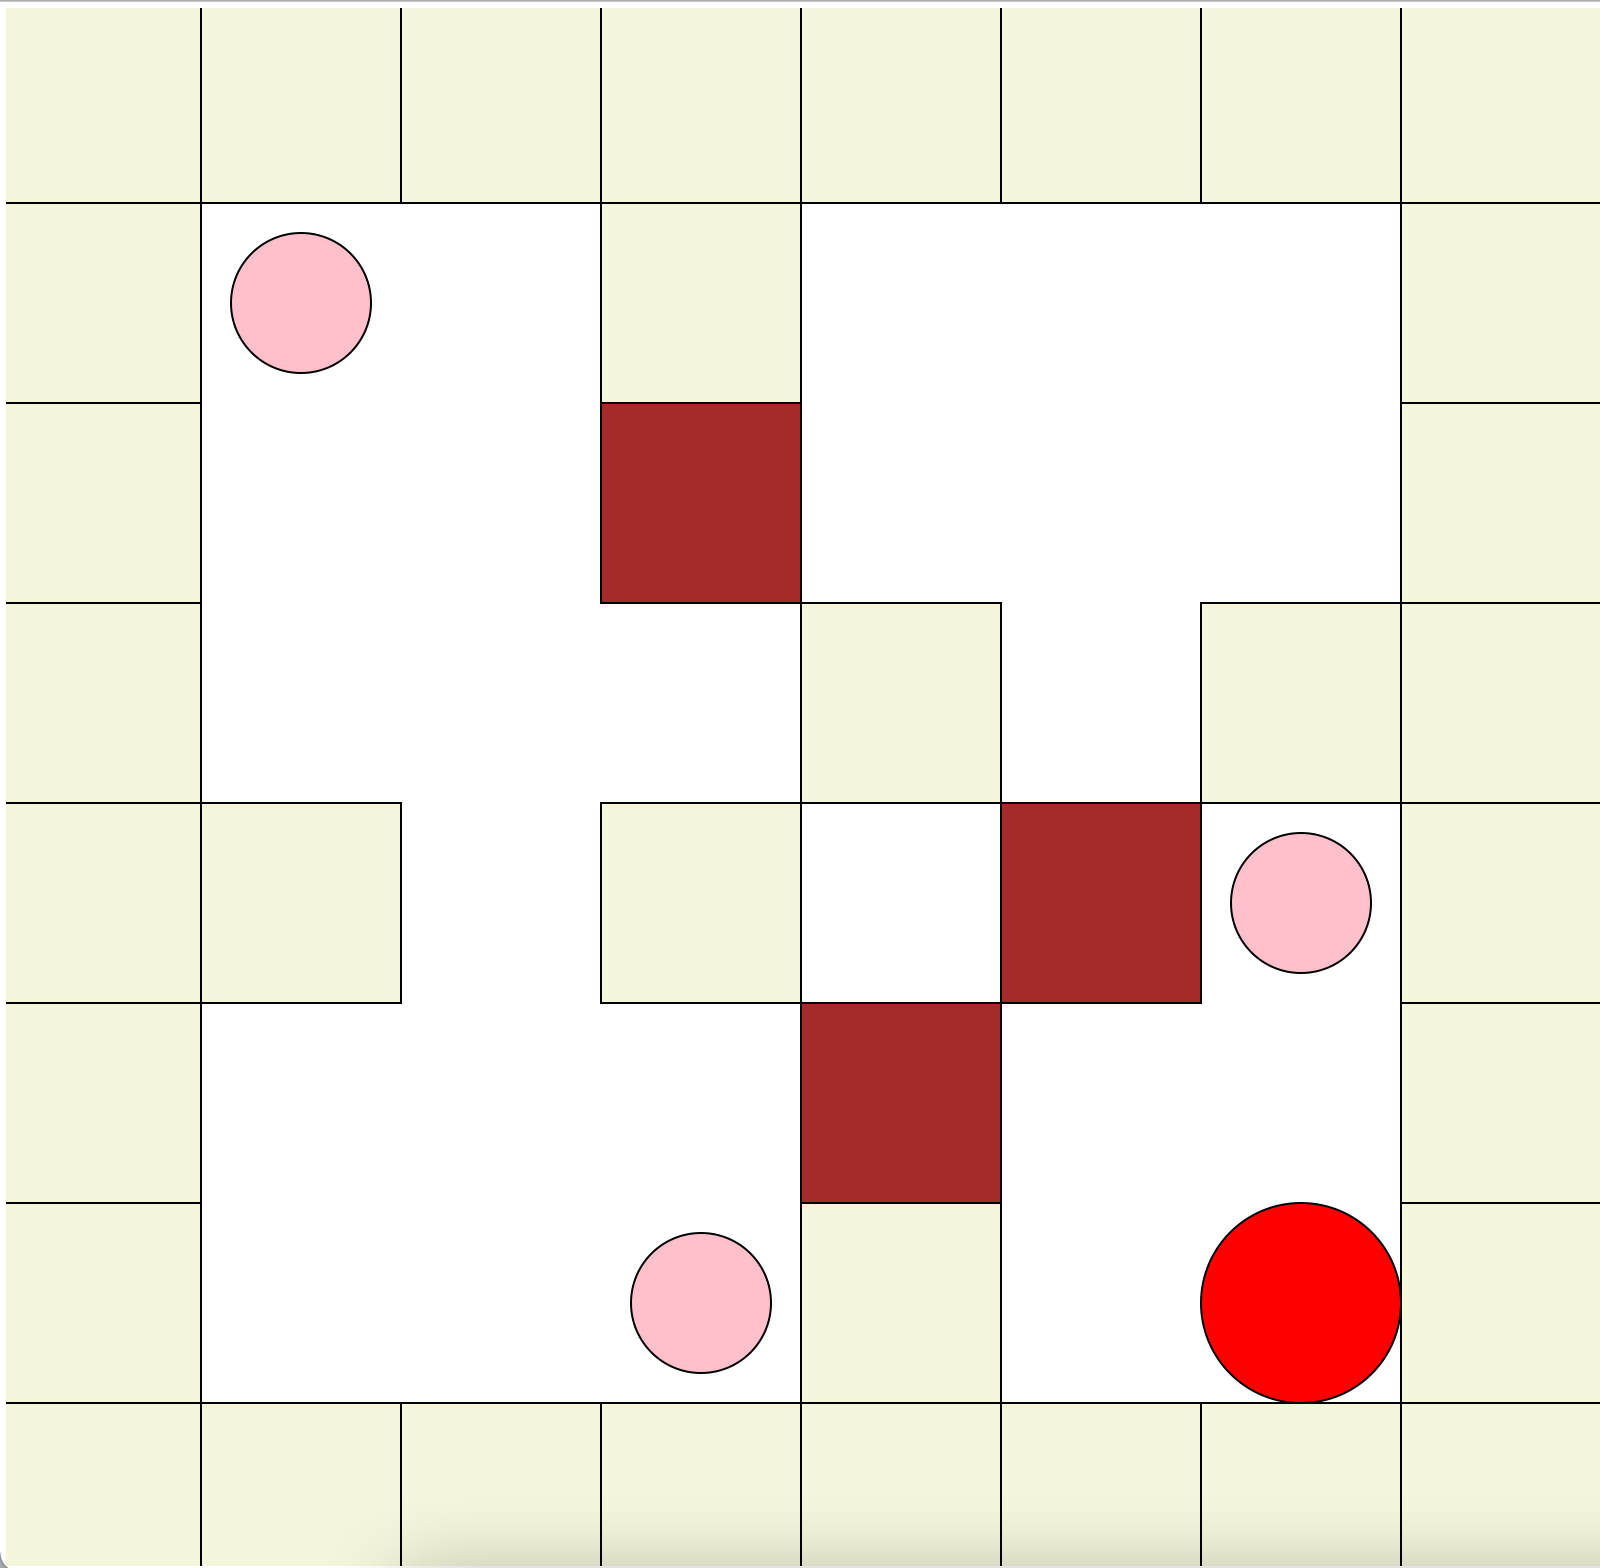
\includegraphics[width=5cm]{Board.png}
        \caption{Initial State of Board}
\end{figure} 
\begin{figure}[htp]
        \centering
        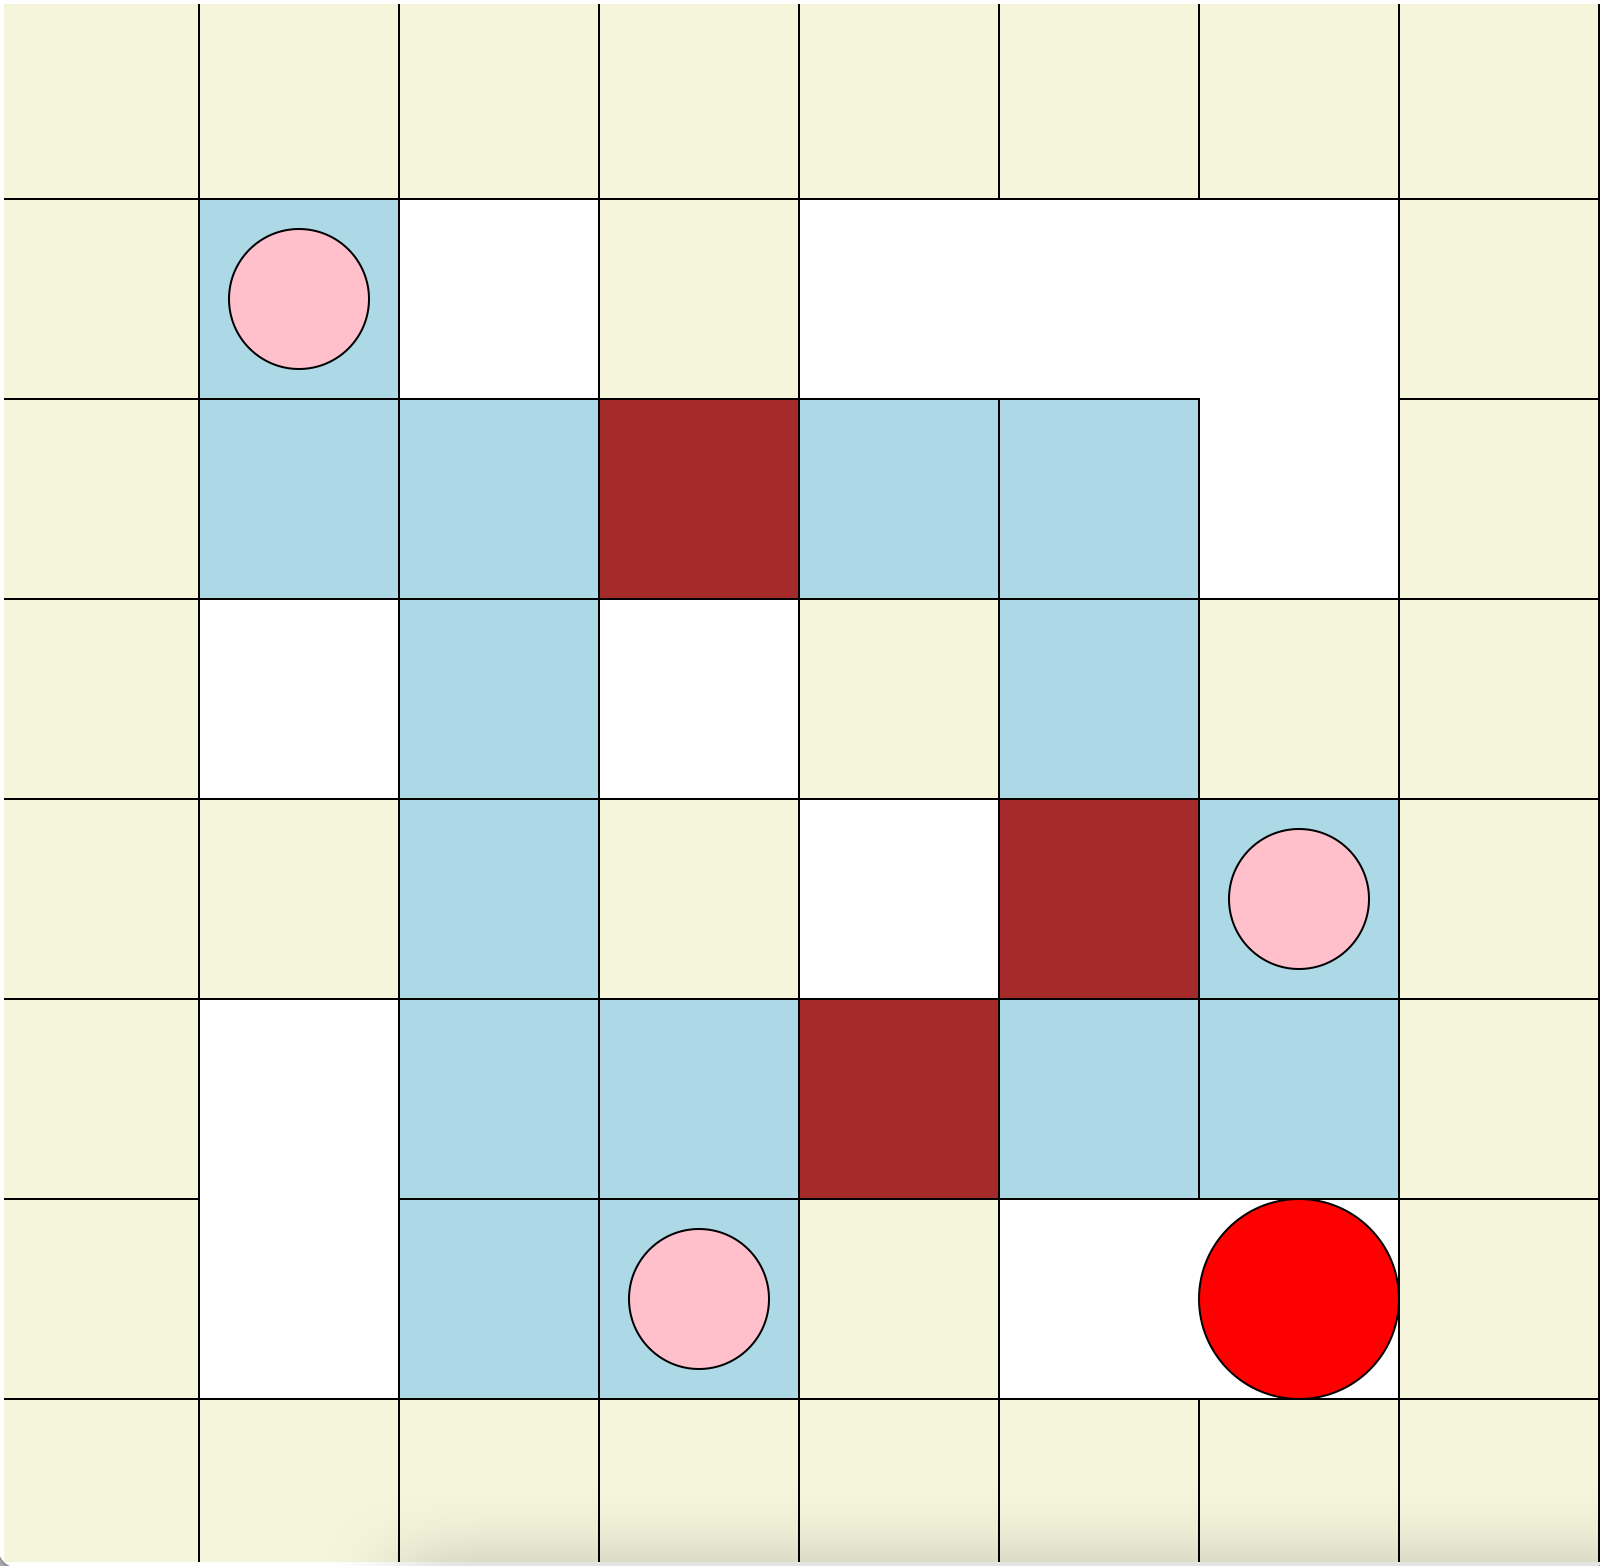
\includegraphics[width=5cm]{Deadlock.png}
        \caption{Blue squares represent safe locations for boxes, white squares represent deadlock locations}
\end{figure} 
\begin{algorithm}
    \caption{Simple Deadlock Detection}\label{euclid}
    \hspace*{\algorithmicindent} \textbf{Input}: location of the box \emph{boxLocation} \\
    \hspace*{\algorithmicindent} \textbf{Output}: recursive call to the Simple Deadlock Function \\
    \begin{algorithmic}
    \State $safeSquares \gets$ a square that does not create an obvious deadlock, initially an empty set
    \State $row, col \gets$ coordinates of the box location \\
    \If{the location of the box is a safe location} 
        \State do nothing
    \EndIf 
    \For{an action in \emph{action} (up, down , left, right)}
        \State $newLocation \gets$ coordinates of the box after taking an action 
        \State $twoStepsLocation \gets$ coordinates of the box after taking the same action twice \\
        \If{\emph{newLocation} within the bounds of the game level \textbf{and} \emph{newLocation} is not a wall \textbf{and} \emph{twoStepsLocation} is not a wall either}
            \State Add \emph{boxLocation} in the list of \emph{safeSquares} % need to figure out how to indent
            \State Call the Simple Deadlock Function with \emph{newLocation} as \underline{input}
        \EndIf
    \EndFor
    \end{algorithmic}
\end{algorithm}

%\textbf{if}
%1) \emph{newLocation} within the bounds of the game level, AND
%2) \emph{newLocation} is not a wall, AND 
%3) \emph{twoStepsLocation} is not a wall either
\newpage
\subsection{Freeze Deadlock Detection Algorithm}

\begin{algorithm}
    \caption{Freeze Deadlock Detection}\label{euclid}
    \hspace*{\algorithmicindent} \textbf{Input}: expected position of the agent \emph{posA} \\
    \hspace*{\algorithmicindent} \textbf{Output}: expected position of the obstacle \emph{posO} \\
    \begin{algorithmic}
    \State $posA \gets$ expected position of the agent
    \State $posO \gets$ expected position of the obstacle \\
    \If{the expected position of obstacle is above \textbf{or} below the expected position of the agent (Vertical Analysis)} 
        \If{the square on the left the agent contain either boxes \textbf{or} walls}
            \State return True
        \ElseIf{the square on the right the agent contain either boxes \textbf{or} walls}
            \State return True
        \Else
            \State return False
        \EndIf
    \ElseIf{ the expected position of obstacle is to the left or right of the expected position of the agent (Horizontal Analysis)}
        \If{the square immediately above the agent contains either boxes \textbf{or} walls}
            \State return True
        \ElseIf{the square immediately below the agent contains either boxes \textbf{or} walls}
            \State return True
        \Else
            \State return False
        \EndIf
    \EndIf 
    \end{algorithmic}
\end{algorithm}

%\emph{posA} $\leftarrow$ expected position of the agent \\ 
%\emph{posO} $\leftarrow$ expected position of the obstacle \\

%\textbf{if} the expected position of obstacle is above or below the expected position of the agent (Vertical Analysis) \\
%(if \emph{posO[0]} $\textless$ \emph{posA[0]} or \emph{posO[0]} $\textgreater$ \emph{posA[0]})

%\textbf{if} the square on the left the agent contain either boxes or walls: return True

%(if \emph{(posA[0], posA[1] - 1)} in self.boxes or \emph{(posA[0], posA[1] - 1)} in self.walls: return True)

%\textbf{elif}  the square on the right the agent contain either boxes or walls: return True

%(elif \emph{(posA[0], pos[1]} + 1) in self.boxes or \emph{(posA[0], posA[1] + 1)} in self.walls: return True)

%\textbf{else} return False
\\
%\textbf{elif} the expected position of obstacle is to the left or right of the expected position of the agent (Horizontal Analysis) \\
%(if \emph{posO[0]} $\textless$ \emph{posA[0]} or \emph{posO[0]} $\textgreater$ \emph{posA[0]})

%\textbf{if} the square immediately above the agent contains either boxes or walls: return True

%(if \emph{(posA[0] - 1, posA[1])} in self.boxes or \emph{(posA[0] - 1, posA[1])} in self.walls: return True)

%\textbf{if} the square immediately below the agent contains either boxes or walls: return True

%(if \emph{(posA[0] + 1, posA[1])} in self.boxes or \emph{(posA[0] + 1, posA[1])} in self.walls: return True)

%\textbf{else} return False
\newpage

\section{Future Considerations}
The Sokoban AI can be improved further with some the following considerations:
\begin{enumerate}
    \item More deadlock detections: Thus far, we have accounted for Simple deadlocks (using pullback DFS strategy), and Freeze deadlocks (using the vertical/horizontal neighborhood search strategy). We can make the agent smarter by identifying more deadlock patterns. In particular, Corral deadlock algorithms would contribute to the game's efficiency.
    \item Macro Moves: Currently our model uses movement in the cardinal directions as actions the agent can take. By defining the actions the agent can take to be macro moves (for example a move could be, move to the nearest box not on a storage location and move it in one of the four directions). This would reduce a lot of time spent in exploration as currently the agent spends a lot of time moving in the board without interacting with any boxes.
    \item Heuristics: The agent moves according to an $\epsilon$-greedy policy so it either moves randomly or according to the policy learned so far. We can use heuristics such as distance to a box and expected number of moves to move a box to a goal to improve the performance of the agent, especially in the early game when most q values are still $0$. 
    \item Deep Q-Learning: As our state (and action) space gets larger as the levels get more complicated, a tabular record of the states and actions can become more and more cumbersome and inefficient. In such scenarios, calling on to deep neural networks to help us generalize across states.
    \item Identifying special cases: Although including a special instance can be very risky in case it fails on higher levels, if we can confidently deduce some universal scenarios and account for them then that might make our algorithm a lot smarter. Nonetheless, we have chosen to not include any such cases as of now so as to push most of our improvements through Q-Learning. 
\end{enumerate}

\section{Random - DELETE LATER}
https://www.researchgate.net/post/Reinforcement-learning-vs-heuristic-search \\
https://github.com/XUHUAKing/sokoban-qlearning/blob/master/sokoban-solver-final-report.pdf \\
https://github.com/XUHUAKing/sokoban-qlearning \\
https://valohai.com/blog/reinforcement-learning-tutorial-basic-deep-q-learning/


\end{document}
